%%%%%%%%%%%%%%%%%%%%%%%%%%%%%%%%%%%%%%%%%
%% Appendix section
% Set-up the section.
\newpage
\appendix
\setcounter{table}{0}
\renewcommand{\thetable}{A\arabic{table}}
\setcounter{figure}{0}
\renewcommand{\thefigure}{A\arabic{figure}}

% Start appendix
\section{Appendix}
\label{appendix}
This project used data which are fully public, and computational tools which are fully open-source.
As such, all code and data (anonymised versions where necessary) involved in this project are available at this project's Github repository, available at \url{https://github.com/shoganhennessy/state-faculty-composition}.
They may be used for replication, or as the basis for further work, as needed.
Any comments or suggestions may be sent to me at \href{mailto:seh325@cornell.edu}{\nolinkurl{seh325@cornell.edu}}, or raised as an issue on the Github project.

A number of statistical packages, for the $R$ language \citep{R2022}, made the empirical analysis for this paper possible.
\begin{itemize}
    \item \textit{Tidyverse} \citep{tidyverse} collected tools for data analysis in the R language.
    \item \textit{LFE} \citep{lfe} implemented linear fixed effect models, with instruments, crucial for the empirical estimation in \autoref{sec:empirics}.
    \item \textit{Stargazer} \citep{stargazer} provided methods to efficiently convert empirical results into presentable output in \LaTeX.
    \item \textit{Lpirfs} \citep{lpirfs2019} implemented estimation of the \cite{jorda2005} local projections methods, with instrumental variables, crucial to the local projections estimates presented in this project.
\end{itemize}

\subsection{IPEDS First Stage}

\begin{table}[H]
    \singlespacing
    %\centering
    \caption{Mean Characteristics for Public Universities, by State Funding Shock Instrument.}
    \makebox[\textwidth][c]{% latex table generated in R 4.3.3 by xtable 1.8-4 package
% Tue Sep 17 11:44:31 2024
\begin{tabular}{lccccc}
  \hline
Instrument Quantile: & 1st & 2nd & 3rd & 4th & 5th \\ 
  \hline
IV Components, \$ per student: &  &  &  &  &  \\ 
  Funding shift--share & -1,473.7 & -2,589.5 & -3,566.4 & -5,002.1 & -8,208.1 \\ 
  Shift in state--wide funding & -6,138.0 & -7,111.6 & -8,593.2 & -10,575.5 & -14,017.6 \\ 
  Share reliance on state funding, \% in 1990--1993 & 25.7 & 37.8 & 42.4 & 47.9 & 59.0 \\ 
  \hline University Funding and Spending, \$ millions: &  &  &  &  &  \\ 
  State funding & 110.3 & 99.2 & 99.8 & 107.1 & 107.1 \\ 
  Tuition revenue & 216.5 & 124.2 & 93.2 & 77.0 & 58.0 \\ 
  Total non-inst. revenues & 355.4 & 241.0 & 203.4 & 190.8 & 169.6 \\ 
  Instruction spending & 219.0 & 139.4 & 108.1 & 100.8 & 92.9 \\ 
  Research Spending & 150.0 & 74.6 & 53.9 & 35.9 & 25.5 \\ 
  \hline University Funding and Spending, \$ per student &  &  &  &  &  \\ 
  State funding & 12,900.1 & 9,956.2 & 9,334.7 & 9,304.9 & 12,766.7 \\ 
  Tuition revenue & 13,129.7 & 8,530.4 & 6,874.6 & 6,046.5 & 5,507.4 \\ 
  Total non-inst. revenues & 30,501.7 & 20,393.8 & 17,194.5 & 15,876.6 & 18,822.8 \\ 
  Instruction spending & 21,680.2 & 12,526.0 & 9,798.1 & 8,482.0 & 9,953.2 \\ 
  Research spending & 16,750.0 & 5,092.8 & 3,327.7 & 2,226.0 & 2,432.4 \\ 
  \hline Selectivity: &  &  &  &  &  \\ 
  Reported enrolment & 14,087.6 & 12,433.8 & 11,328.8 & 11,546.2 & 10,252.9 \\ 
  Full-time equivalent enrolment & 12,452.8 & 10,597.3 & 9,638.4 & 9,876.6 & 8,554.9 \\ 
  Acceptance rate, \% & 70.7 & 73.2 & 70.8 & 64.5 & 60.2 \\ 
  6 Year graduation rate, \% & 55.6 & 47.3 & 44.1 & 44.7 & 45.2 \\ 
   \hline
\end{tabular}
}
    \label{tab:summary-quantiles}
    \justify
    \footnotesize
    \textbf{Note}:
    This table shows the summary statistics for every public university--year observation in IPEDS data, for each of the 5 quantiles of the funding shock instrument.
    The column labelled ``1st'' refers to the mean for all university-year observations in the first quintile (bottom 20\%) of the funding shock distribution, and so on.
    The numbers are adjusted to 2021 figures by CPI-U.
    Non-institutional revenues refers to the sum of federal, state, and local funding plus tuition revenues; these sum to the majority of university funding, but exclude numbers such as university income from capital projects.
\end{table}

\begin{figure}[H]
    \centering
    \singlespacing
    \caption{Correlation Between State Funding Shock and Public University State Funding in Surrounding Years.}
    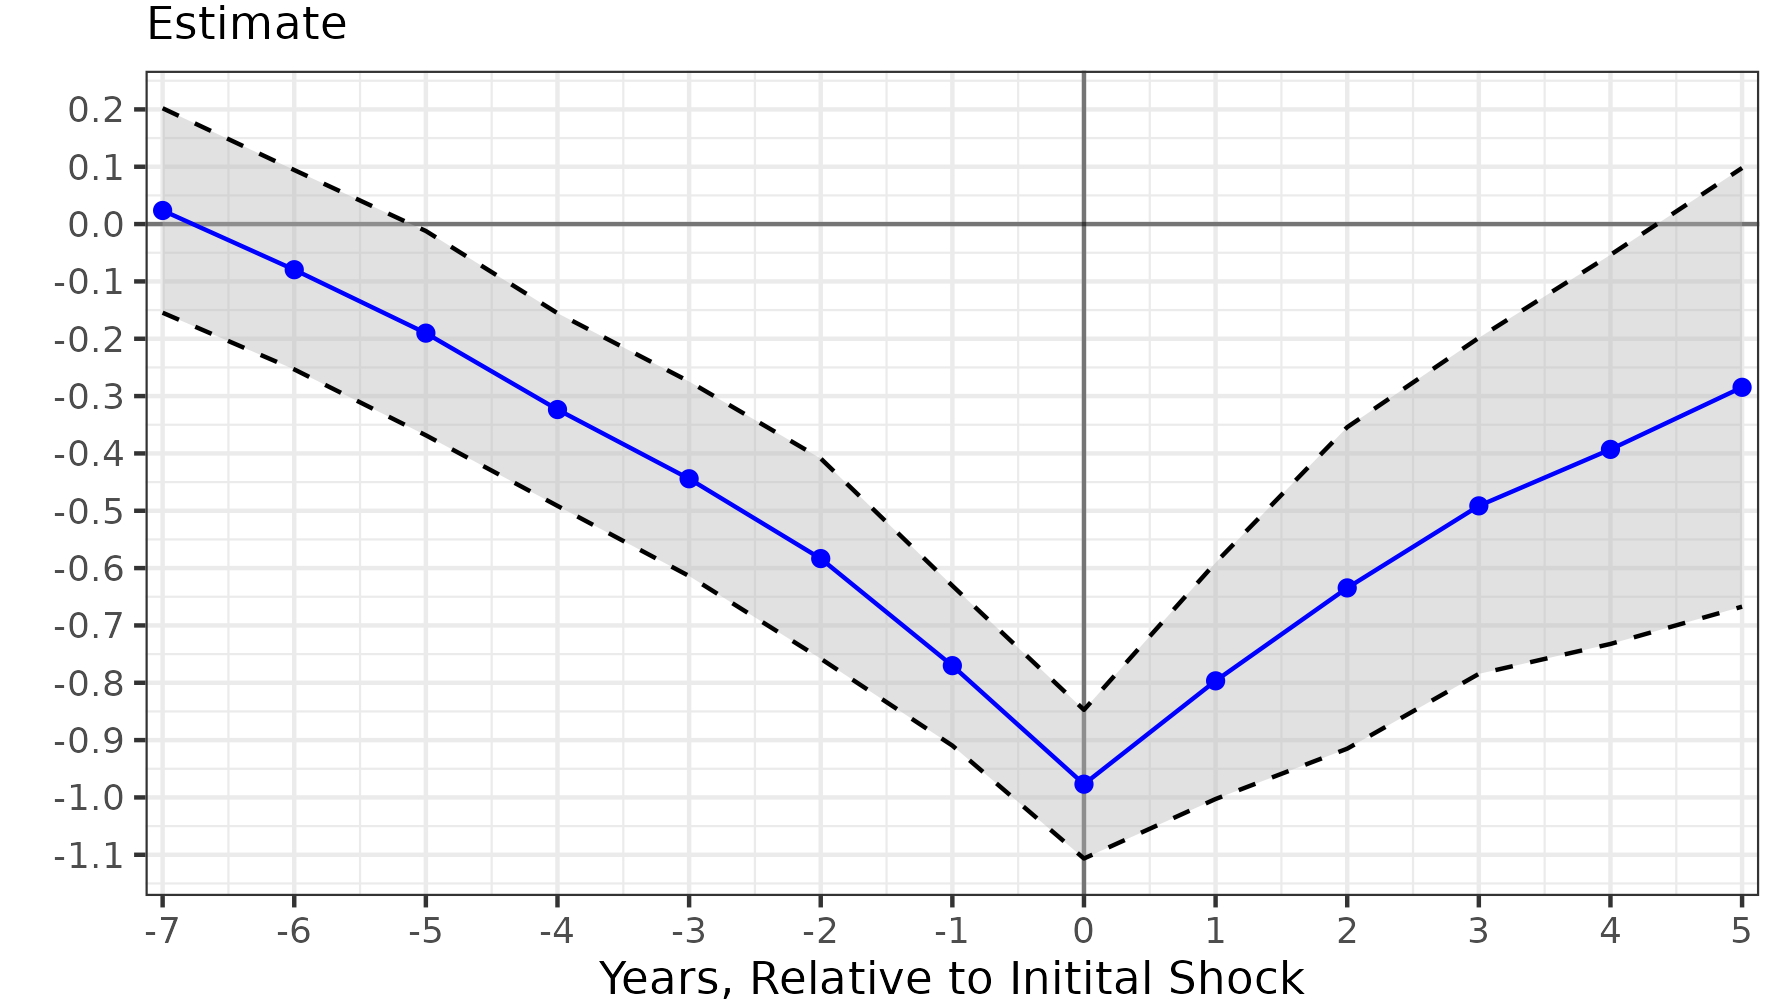
\includegraphics[width=\textwidth]{figures/lag-firststage.png}
    \label{fig:lag-firststage}
    \justify
    \footnotesize
    \textbf{Note}:
    This figure shows the correlation between state funding in year $t+k$ with the funding shock in year $t$ for a university, where $k = -7, \hdots, 5$ are the years on the x-axis.
    This shows that state funding and the funding shock have dynamic correlation, so that dynamic effects must be estimated by local projections -- and not simple OLS or 2SLS.
    The estimates are of \eqref{eqn:firststage}, calculated with IPEDS data, separately for each year relative to initial shock, using the $\log-\log$ specification, including fixed effects for university $+$ year, and clustering standard errors by university $+$ year.
\end{figure}

\begin{figure}[H]
    \centering
    \singlespacing
    \caption{Local Projection Estimates for Funding Shock on State Funding, in IPEDS Data.}
    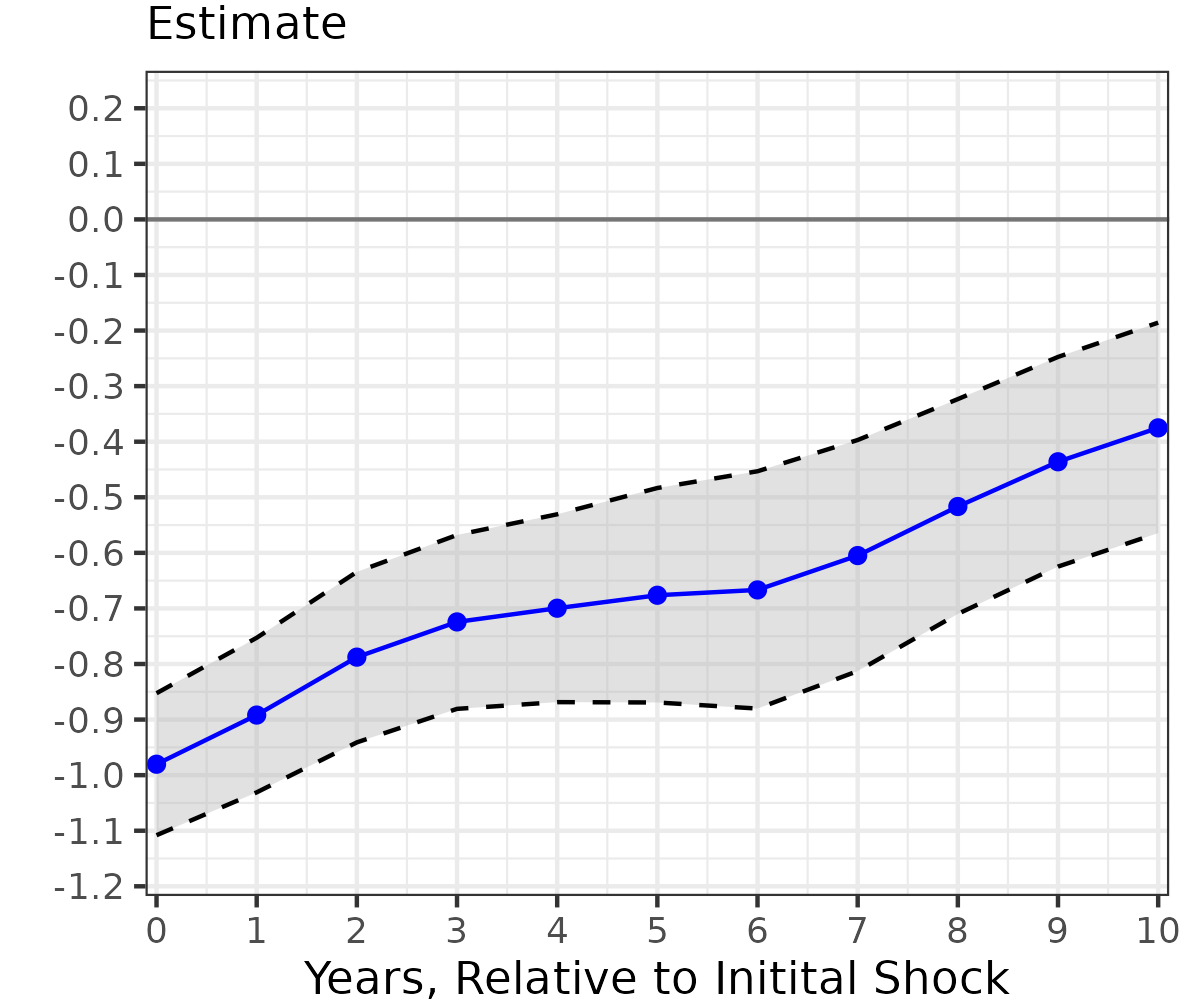
\includegraphics[width=0.6\textwidth]{figures/firststage-lp.png}
    \label{fig:firststage-lp}
    \justify
    \footnotesize
    \textbf{Note}:
    These figures show the local projections estimates of regression specification \eqref{eqn:firststage}, with the funding shock as an instrument for state funding, using IPEDS data.
    The coefficient estimate is effect of funding shock ($Z_{i,t}$) on state funding ($X_{i,t}$), while accounting for auto-correlation between different time periods --- i.e., between $Z_{i,t}, Z_{i,t-1}$ and $X_{i,t}, X_{i,t-1}$.
    These results use a $\log-\log$ specification, so the estimates are for the elasticity of state funding per student in a year $t+k$ with respect to funding shock in year $t$, where years $k = 0, \hdots, 10$ are on the x-axis. 
    Standard errors are clustered at the state-year level.
\end{figure}

\newpage
\subsection{Illinois IBHED First Stage}
\label{sec:iv-model-indiv}

This paper uses data on individual professors in the Illinois university system, to investigate the effects of changes in university revenues on the individual professors at the universities.
The outcomes here now refer to individual professors (e.g., their salary and promotion rate), so requires adjustment to the empirical approach, leveraging variation in university funding for the years after a professor joins the university.

\autoref{eqn:rolling-instrument} defines a rolling-share variant of the instrument, $\tilde Z_{j,t}$, where the university's state funding share exposure is based in the year a professor joins the university --- and not the base period 1990--1993.
$j$ indexes each professor in year $t$, $\tau(j)$ for the year the professor first joins their institution.
Identifying $\tau(j)$ is possible for $j$ by restricting to all professors hired 2011-2021 --- i.e., in the years after the start of the full panel.
It is not possible to discern the hiring year for professors who  were hired in the years preceding 2011, and so the entire sample is only possible to analyse using the base-share in years 1990-1993 formulation.

\begin{align}
    \label{eqn:rolling-instrument}
    \tilde Z_{j,t} &\coloneqq - \left[
    \left( \frac{\text{Total State Funding}_{s(j),t}}{\text{Student Population}_{s(j),t}} \right)
    \left( \frac{\text{State Funding}_{\tau(j)}}{\text{Total Revenues}_{i,\tau(j)}} \right) \right]
\end{align}

This approach leverages an insight, made available by level of the data: that an individual professor is affected by changes in university revenues after they have joined the university.
\autoref{sec:iv-model-uni} considers the number of professors employed by the university; whether a professor becomes employed at the university is likely affected by that university's finances.
The formulation here takes as given that the professor is already employed at the university, and then projects the effect of changes in state funding on these \textit{incumbent} professors following the state funding shock.

Exogeneity and relevance of the rolling-share instrument, $\tilde Z_{j,t}$, follows the same reasoning as that for the base-share instrument, $Z_{i,t}$, discussed in \autoref{sec:approp-shocks}.
The base-share instrument is appropriate for some outcomes with the individual Illinois professors, where appropriate.
We satisfy the assumptions for exogeneity by noting that none of the Illinois public campuses take the majority of state funding, and that the identification strategy relies on exogeneity in changes in state funding to individual professor-outcomes, following the year they joined the university.
Additionally, within-institution changes resulting from share reliance on state funding may be correlated with unobserved changes in the outcomes, so that \cite{NBERw27885} note the importance of controlling for the base share and state student population.
The formulation here implicitly controls for these factors via the fixed effects; results are relatively similar while including these controls with and without including fixed effects, and so are omitted.

The instrumental variables model is then defined as follows, where $i(j)$ refers to the institution that professor $j$ is employed at, and $Y_{j,t}$ for salary, rate of promotion, and propensity to leave the Illinois public university system.
The system includes fixed effects for the institution and first year of employment.
The instrument varies by institution, based in the year of first employment, so that these are the corresponding fixed effects and level of clustered standard errors.
\begin{eqnarray}
    \label{eqn:secondstage1_indiv}
    X_{i(j),t} &=& \theta_{i(j)} + \phi_{\tau(j)} + \delta \tilde Z_{i(j),t} + \epsilon_{i(j),t} \\
    \label{eqn:secondstage2_indiv}
    Y_{j,t} &=& \mu_{i(j)} + \nu_{\tau(j)} + \beta \widehat X_{i(j),t} + \varepsilon_{j,t}
\end{eqnarray}
We then interpret parameter $\beta$ as the effect of changes in state funding at an Illinois public university, via state funding shocks, on an individual professor's outcome $Y_{j,t}$.

\newpage
\begin{figure}[H]
    \centering
    \singlespacing
    \caption{Local Projection Estimates for Effect of State Funding on Faculty Promotion Rate at Illinois Public Universities, by Professor Group.}
    \begin{subfigure}[b]{0.495\textwidth}
        \centering
        \caption{Lecturers.}
        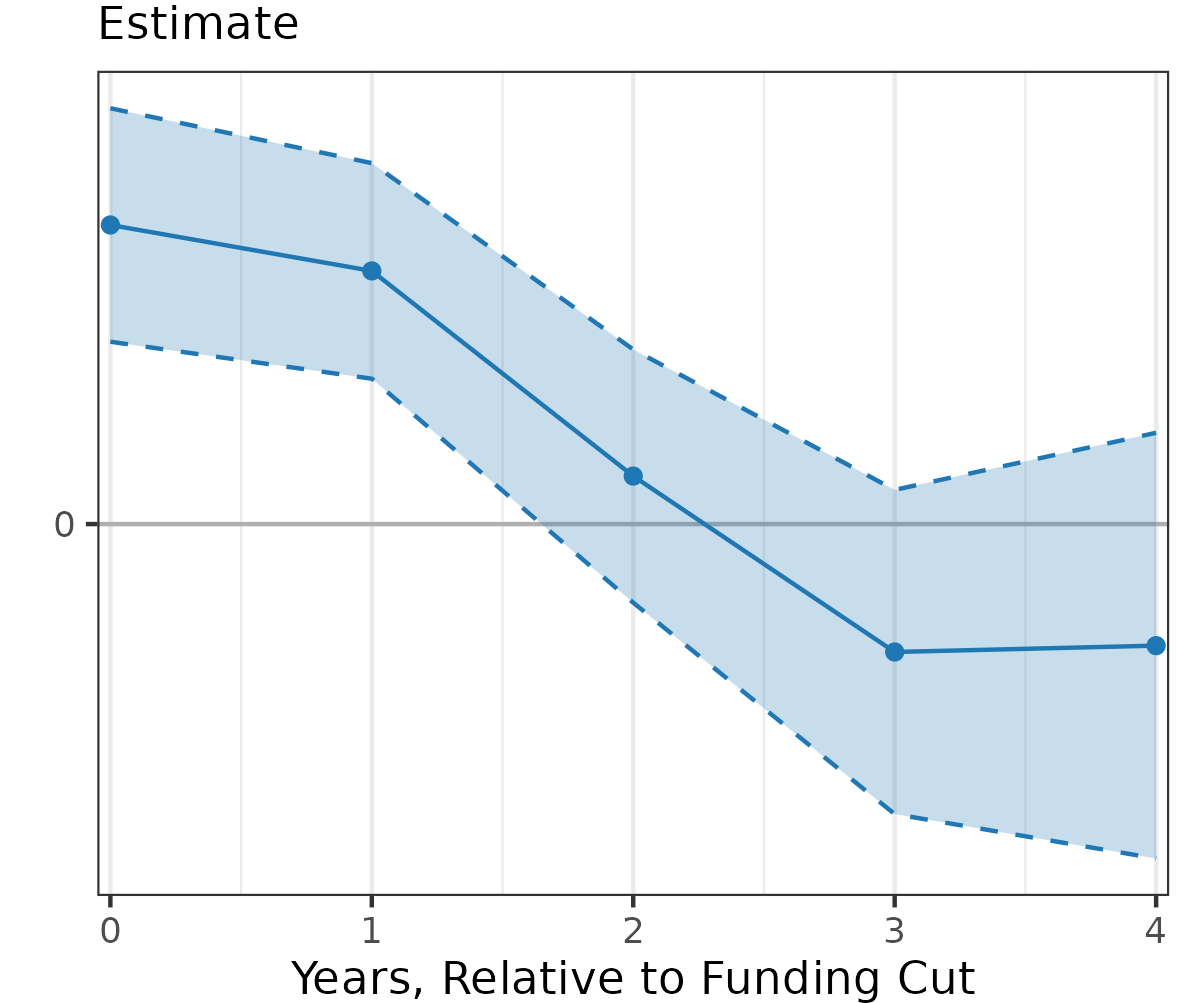
\includegraphics[width=\textwidth]{figures/promoted-lecturer-illinois-lp-rolling.png}
        \label{fig:promoted-lecturer-illinois-lp-rolling}
    \end{subfigure}
    \begin{subfigure}[b]{0.495\textwidth}
        \centering
        \caption{Assistant Professors.}
        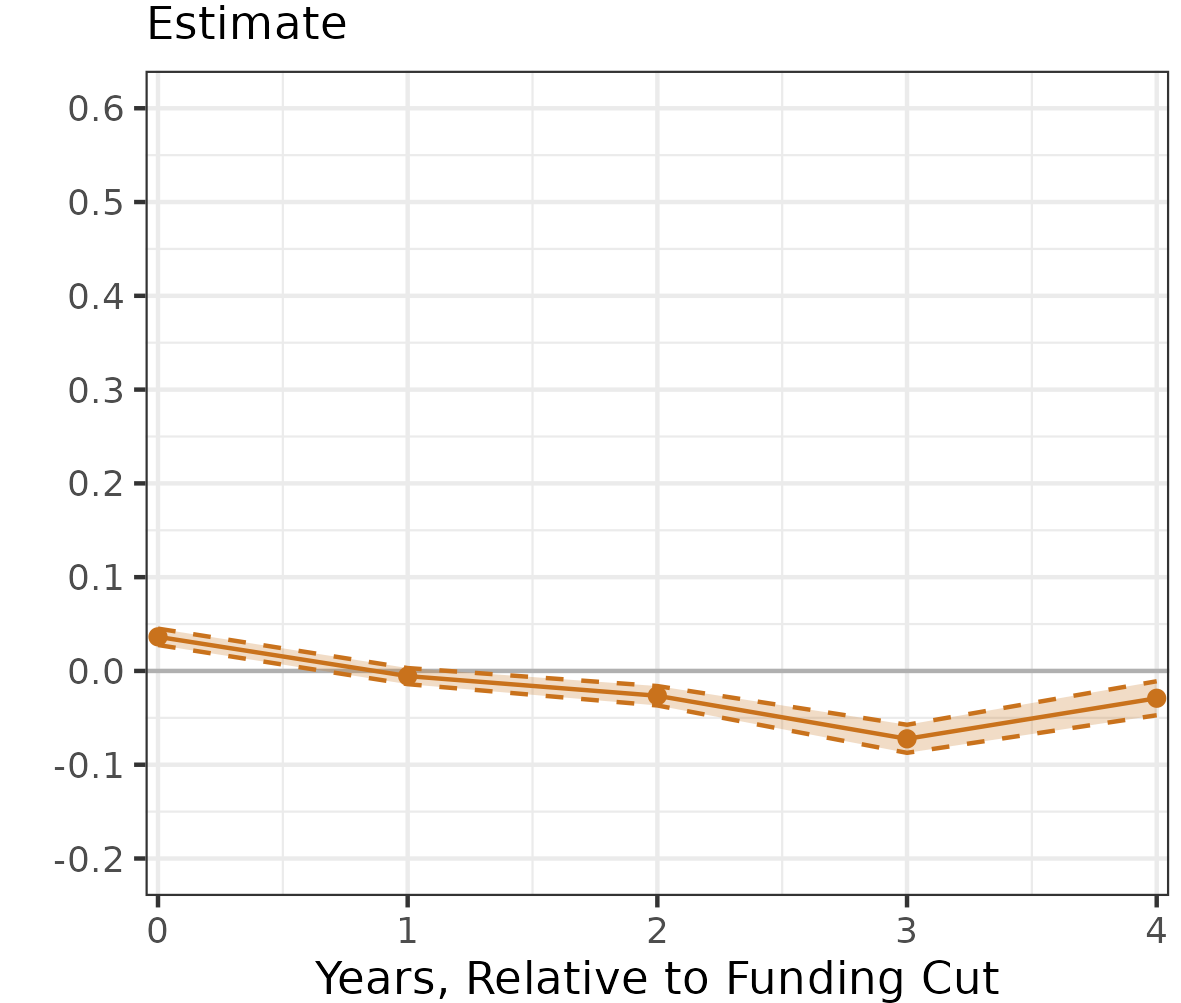
\includegraphics[width=\textwidth]{figures/promoted-assistant-illinois-lp-rolling.png}
        \label{fig:promoted-assistant-illinois-lp-rolling}
    \end{subfigure}
    \begin{subfigure}[b]{0.495\textwidth}
        \centering
        \caption{Full Professors.}
        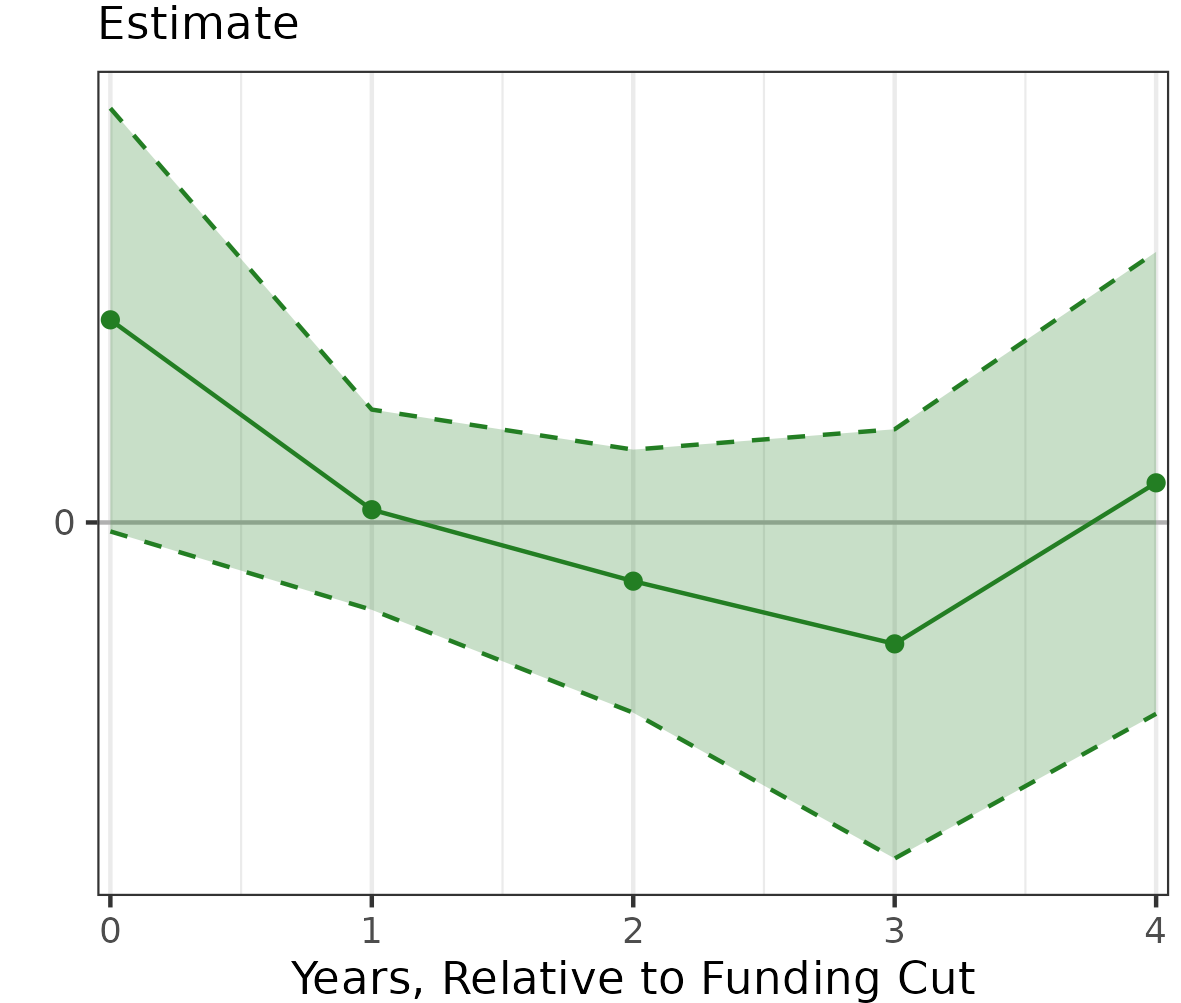
\includegraphics[width=\textwidth]{figures/promoted-full-illinois-lp-rolling.png}
        \label{fig:promoted-full-illinois-lp-rolling}
    \end{subfigure}
    \label{fig:promoted-illinois-lp-rolling}
    \justify
    \footnotesize
    \textbf{Note}:
    These figures show the local projections estimates of regression specification \eqref{eqn:secondstage}, with the funding shock as an instrument for state funding.
    The unit of analysis is an individual faculty member (at an Illinois public university); funding data come from IPEDS, and faculty promotion rate from IBHED.
    The coefficient estimate is effect of state funding ($X_{i(j),t}$) on faculty promotion rate ($Y_{j,t}$), while accounting for auto-correlation between different time periods --- i.e., between $X_{i(j),t}, X_{i(j),t-1}$ and $Y_{i(j),t}, Y_{i(j),t-1}$.
    These results use a rate$-\log$ specification, so the estimates are for the rate of promotion in a year $t+k$ affected by a 1\% change in state funding in year $t$, where years $k = 0, \hdots, 4$ are on the x-axis. 
    Standard errors are clustered at the university-year level.
\end{figure}

\newpage
\begin{figure}[H]
    \centering
    \singlespacing
    \caption{Local Projection Estimates for Effect of State Funding on Faculty Exit Rate at Illinois Public Universities, by Professor Group.}
    \begin{subfigure}[b]{0.495\textwidth}
        \centering
        \caption{Lecturers.}
        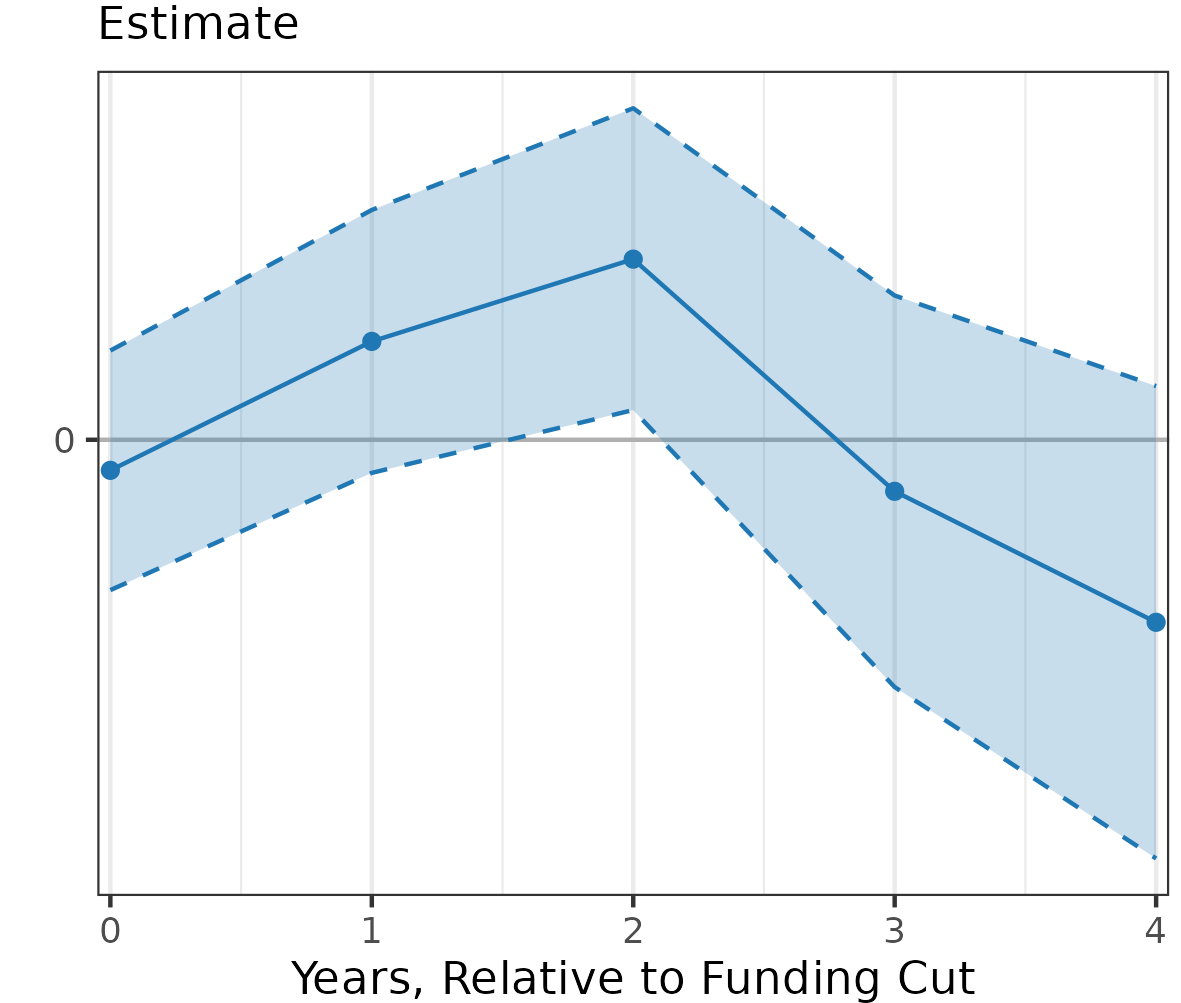
\includegraphics[width=\textwidth]{figures/exit-lecturer-illinois-lp-rolling.png}
        \label{fig:exit-lecturer-illinois-lp-rolling}
    \end{subfigure}
    \begin{subfigure}[b]{0.495\textwidth}
        \centering
        \caption{Assistant Professors.}
        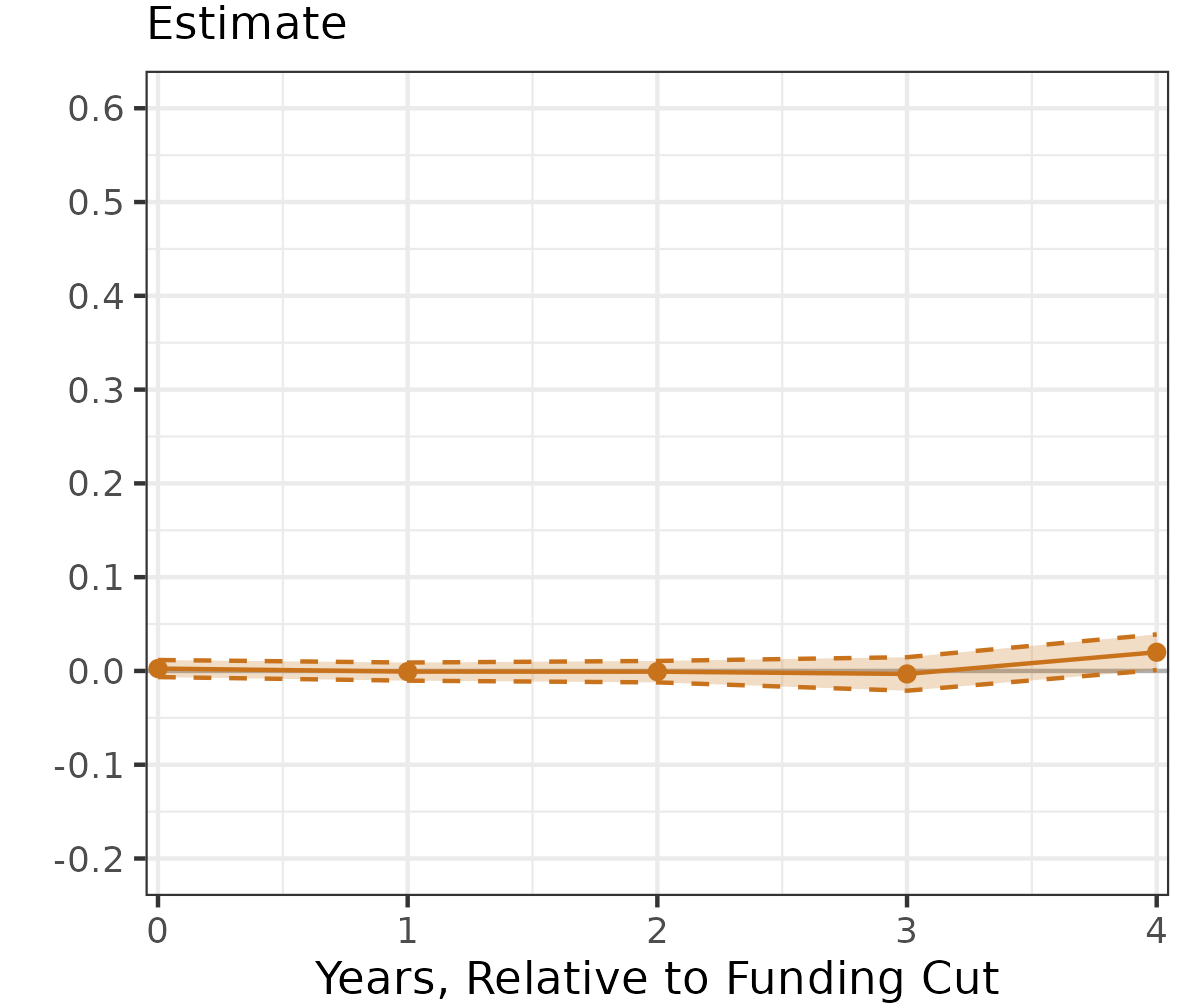
\includegraphics[width=\textwidth]{figures/exit-assistant-illinois-lp-rolling.png}
        \label{fig:exit-assistant-illinois-lp-rolling}
    \end{subfigure}
    \begin{subfigure}[b]{0.495\textwidth}
        \centering
        \caption{Full Professors.}
        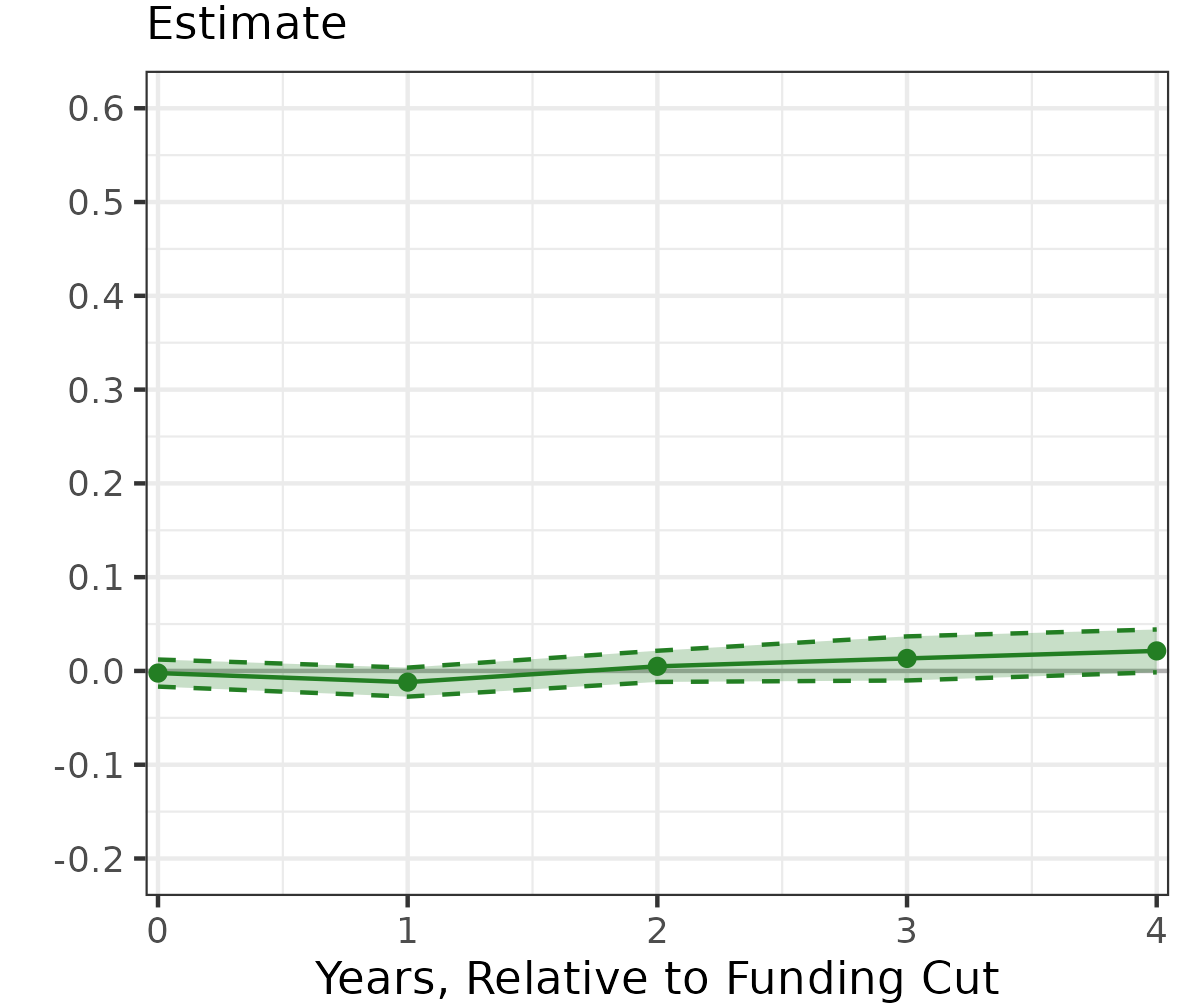
\includegraphics[width=\textwidth]{figures/exit-full-illinois-lp-rolling.png}
        \label{fig:exit-full-illinois-lp-rolling}
    \end{subfigure}
    \begin{subfigure}[b]{0.495\textwidth}
        \centering
        \caption{Administrator Professors.}
        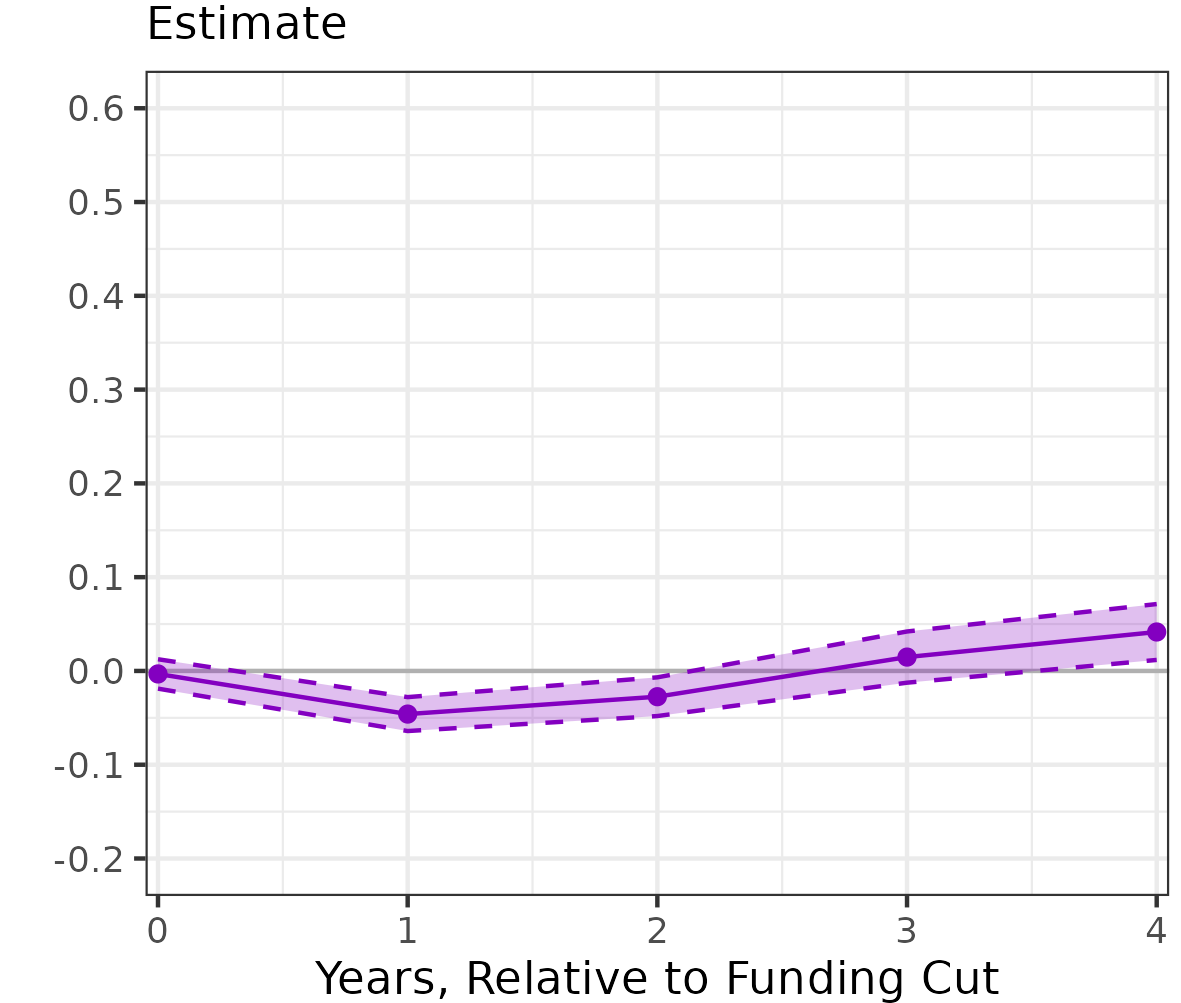
\includegraphics[width=\textwidth]{figures/exit-administrator-illinois-lp-rolling.png}
        \label{fig:exit-administrator-illinois-lp-rolling}
    \end{subfigure}
    \label{fig:exit-illinois-lp-rolling}
    \justify
    \footnotesize
    \textbf{Note}:
    These figures show the local projections estimates of regression specification \eqref{eqn:secondstage}, with the funding shock as an instrument for state funding.
    The unit of analysis is an individual faculty member (at an Illinois public university); funding data come from IPEDS, and faculty promotion rate from IBHED.
    The coefficient estimate is effect of state funding ($X_{i(j),t}$) on faculty promotion rate ($Y_{j,t}$), while accounting for auto-correlation between different time periods --- i.e., between $X_{i(j),t}, X_{i(j),t-1}$ and $Y_{i(j),t}, Y_{i(j),t-1}$.
    These results use a rate$-\log$ specification, so the estimates are for the rate of promotion in a year $t+k$ affected by a 1\% change in state funding in year $t$, where years $k = 0, \hdots, 4$ are on the x-axis. 
    Standard errors are clustered at the university-year level.
\end{figure}




\newpage
\subsection{Additional Results, Faculty Hiring}
\label{sec:appendix-hiring}

These results were produced by integrating the total count of faculty hires for 2010--2021 for the top-ranked 180 US universities with a sum of the funding variables, and then estimating the models specified in \autoref{sec:iv-model-uni}.
There were no observable differences in the hiring rate of male vs female faculty.

\begin{figure}[h!]
    \centering
    \singlespacing
    \caption{State Funding and Faculty Hired at Public Universities, Total for 2011--2021.}
    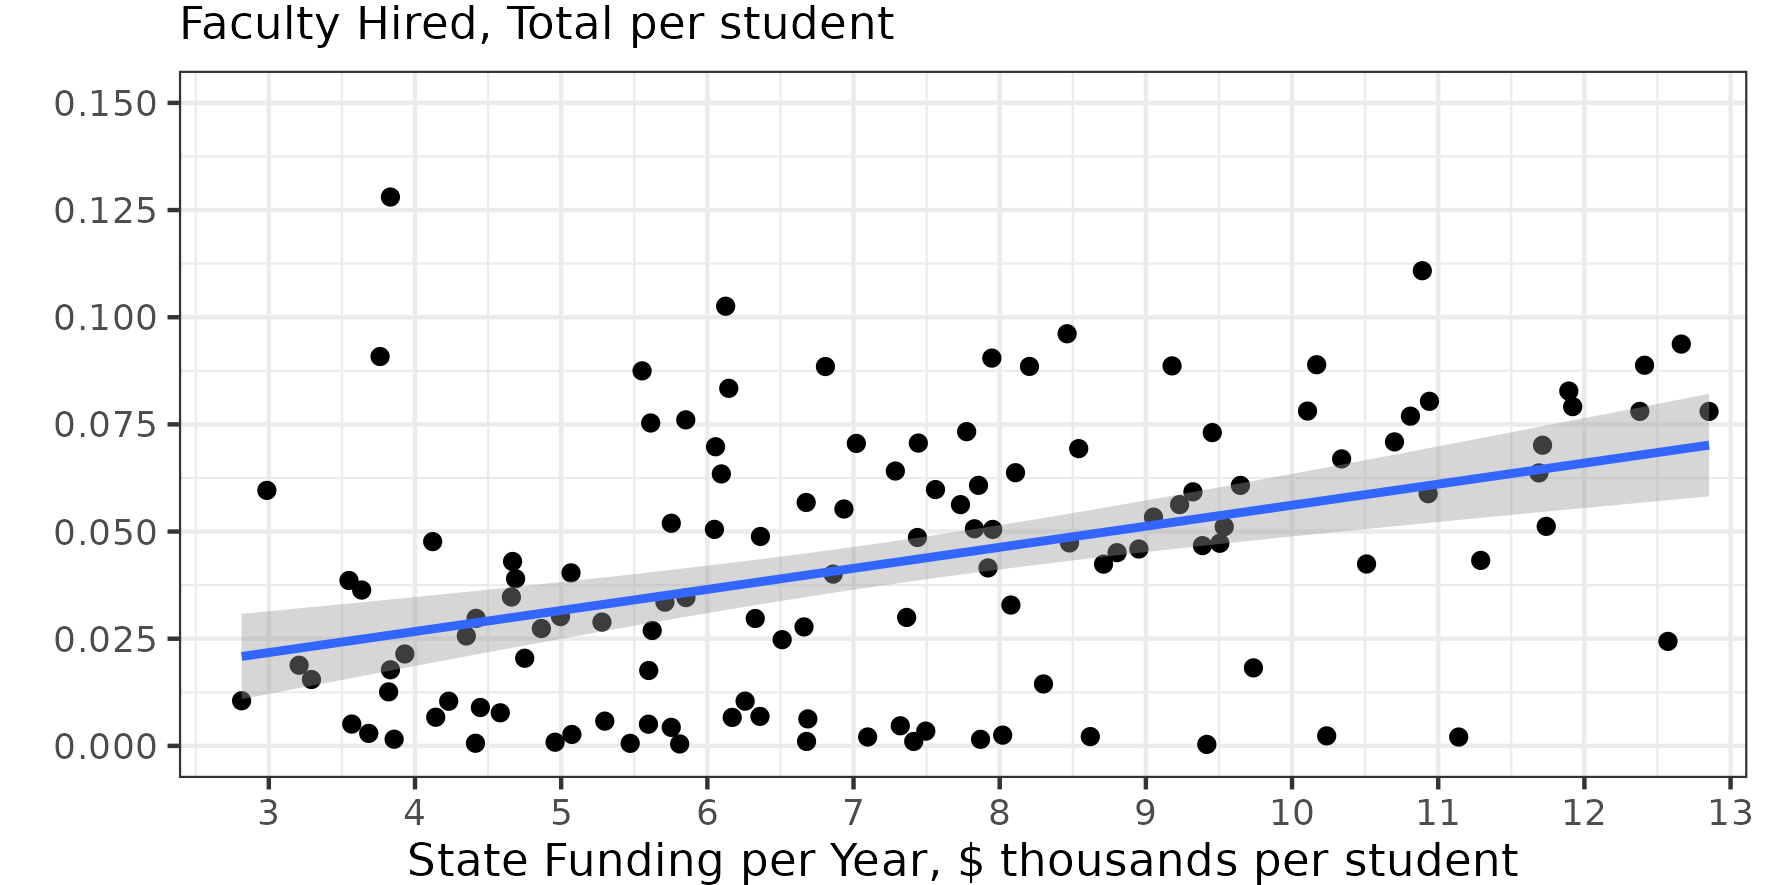
\includegraphics[width=0.8\textwidth]{figures/hiring-correlation.png}
    \label{fig:hiring-correlation}
    \justify
    \footnotesize
    \textbf{Note}:
    This figure shows the correlation between state funding and the number of total number of faculty hired at public universities between 2011--2021, and the line is a line of best-fit.
    Data for the number of faculty hired at public universities are provided by \cite{wapman2022quantifying}, and funding data from IPEDS.
\end{figure}

\newpage
\begin{table}[h!]
    \singlespacing
    \centering
    \caption{OLS and 2SLS Estimates for University Faculty Hires, in Illinois 2011--2021.}

    \textbf{Panel A: units in \$ per student}

    \makebox[\textwidth][c]{
\begin{tabular}{@{\extracolsep{5pt}}lcccccccc} 
\\[-1.8ex]\hline 
\hline \\[-1.8ex] 
 & \multicolumn{8}{c}{Dependent Variable: Yearly New Hires by Professor Group} \\ 
\cline{2-9} 
\\[-1.8ex] & \multicolumn{2}{c}{Lecturers} & \multicolumn{2}{c}{Asst. Professors} & \multicolumn{2}{c}{Full Professors} & \multicolumn{2}{c}{All Faculty} \\ 
 & OLS & 2SLS & OLS & 2SLS & OLS & 2SLS & OLS & 2SLS \\ 
\\[-1.8ex] & (1) & (2) & (3) & (4) & (5) & (6) & (7) & (8)\\ 
\hline \\[-1.8ex] 
 State Funding & $-$2.551 & $-$2.280 & 0.060 & $-$5.126 & $-$0.095 & $-$2.562 & $-$2.677 & 23.012 \\ 
  & (1.420) & (9.168) & (0.675) & (7.210) & (0.249) & (7.051) & (2.185) & (52.652) \\ 
 \hline \\[-1.8ex] 
Outcome Mean & 73.275 & 73.275 & 42.771 & 42.771 & 12.301 & 12.301 & 151.932 & 151.932 \\ 
Observations & 131 & 131 & 131 & 131 & 113 & 113 & 132 & 132 \\ 
R$^{2}$ & 0.839 & 0.839 & 0.934 & 0.902 & 0.788 & 0.752 & 0.918 & 0.793 \\ 
\hline 
\hline \\[-1.8ex] 
\end{tabular} 
}
    
    \textbf{Panel B: units in log \$ per student}
    
    \makebox[\textwidth][c]{
\begin{tabular}{@{\extracolsep{5pt}}lcccccccc} 
\\[-1.8ex]\hline 
\hline \\[-1.8ex] 
 & \multicolumn{8}{c}{Dependent Variable: Employment Count} \\ 
\cline{2-9} 
\\[-1.8ex] & \multicolumn{2}{c}{Lecturers} & \multicolumn{2}{c}{Asst. Professors} & \multicolumn{2}{c}{Full Professors} & \multicolumn{2}{c}{All Faculty} \\ 
 & OLS & 2SLS & OLS & 2SLS & OLS & 2SLS & OLS & 2SLS \\ 
\\[-1.8ex] & (1) & (2) & (3) & (4) & (5) & (6) & (7) & (8)\\ 
\hline \\[-1.8ex] 
 State Funding & 0.120 & 0.158 & 0.172 & 0.174 & 0.191 & 0.235 & 0.046 & 0.082 \\ 
  & (0.071) & (0.065) & (0.154) & (0.143) & (0.113) & (0.137) & (0.080) & (0.047) \\ 
 \hline \\[-1.8ex] 
Outcome Mean & 0.494 & 0.494 & 0.234 & 0.234 & 0.051 & 0.051 & 0.993 & 0.993 \\ 
Observations & 131 & 131 & 131 & 131 & 113 & 113 & 132 & 132 \\ 
R$^{2}$ & 0.749 & 0.749 & 0.482 & 0.482 & 0.628 & 0.627 & 0.580 & 0.579 \\ 
\hline 
\hline \\[-1.8ex] 
\end{tabular} 
}
    \label{tab:facultyhires-illinois-reg}
    \justify
    \footnotesize
    \textbf{Note}:
    These tables show the second stage OLS and 2SLS estimates of regression specification \eqref{eqn:secondstage}, showing the effect of state funding changes on number of faculty hires at Illinois universities, using the funding shock to instrument for state funding in the columns labelled 2SLS.
    Each observation is a public university-year in the state of Illinois, where funding data come from IPEDS and faculty count come from IBHED data.
    Panel A shows the effect of a fall in state funding \$-1,000 per student in the state on the number of new faculty hires by position.
    Panel B shows the effect of a $10$\% change in state funding per student at the university on the 10\% change in the number of faculty hires per students.
    Outcome-mean is the mean of the outcome, for Panel A the number of faculty hires, for Panel B the number of faculty hires per student.
    Panel B uses $\log$ new faculty hires per student as the outcome, though the outcome mean is count of new faculty hires  per student (not in $\log$ terms).
    Standard errors are clustered at the university-year level, and university $+$ year fixed effects are included through--out.
\end{table}

Yearly variation is not observed here, so that only the aggregate level, for 180 universities, can be considered.
\begin{table}[H]
    \singlespacing
    \centering
    \caption{OLS and 2SLS Estimates for University Faculty Hiring, Total for 2011--2020.}
    \makebox[\textwidth][c]{
\begin{tabular}{@{\extracolsep{5pt}}lcccccc} 
\\[-1.8ex]\hline 
\hline \\[-1.8ex] 
 & \multicolumn{6}{c}{Dependent Variable: Professor Hiring Count} \\ 
\cline{2-7} 
\\[-1.8ex] & \multicolumn{2}{c}{Men} & \multicolumn{2}{c}{Women} & \multicolumn{2}{c}{Total} \\ 
 & OLS & 2SLS & OLS & 2SLS & OLS & 2SLS \\ 
\\[-1.8ex] & (1) & (2) & (3) & (4) & (5) & (6)\\ 
\hline \\[-1.8ex] 
 State Funding & 0.805 & 1.308 & 0.845 & 1.325 & 0.848 & 1.306 \\ 
  & (0.222) & (0.365) & (0.235) & (0.335) & (0.220) & (0.352) \\ 
 \hline \\[-1.8ex] 
Observations & 157 & 157 & 157 & 157 & 157 & 157 \\ 
R$^{2}$ & 0.396 & 0.366 & 0.415 & 0.383 & 0.408 & 0.381 \\ 
\hline 
\hline \\[-1.8ex] 
\end{tabular} 
}
    \label{tab:hiring-shock-reg}
    \justify
    \footnotesize
    \textbf{Note}: 
    This table show the second stage 2SLS estimates of regression specification \eqref{eqn:secondstage}, showing the effect of state funding changes on the number of faculty hires (per student) total for 2011--2021 at US public universities, using the funding shock to instrument for state funding.
    Each observation is a university--year at a public university, where funding data come from IPEDS and faculty count total for 2011--2021 from \citep{wapman2022quantifying}.
    The panels show the effect of a $1$\% change in state funding per student at the university (total for 2011--2021) on the number of new faculty hires by gender (and all).
    Standard errors are clustered at the university-year level, and university $+$ year fixed effects are included through--out.
\end{table}


\newpage
\subsection{Additional Results, Rates of Substitution}
\label{sec:appendix-substitution}

The funding elasticities can be used to recover the marginal rate of substitution between two outcomes.
For example, write $Y^1$ for the number of lecturers per student at a university, and $Y^2$ for the number of full professors.
I use the above approaches to estimate the funding elasticities, where $\% \Delta$ denotes percent change.
\[ \beta_1 = \frac{\% \Delta Y^1}{\% \Delta X}
\text{, and }
\beta_2 = \frac{\% \Delta Y^2}{\% \Delta X} \]
As such, it is possible to recover the elasticity for substitution between lecturers and full professors by the universities via the respective funding elasticities.
\[ \frac{\% \Delta Y^1}{\% \Delta Y^2}
= \frac{\% \Delta Y^1 / \% \Delta X}{\% \Delta Y^2 / \% \Delta X}
= \frac{\beta_1}{\beta_2} \]
I present results for the rates of substitution between different levels of faculty by this approach, dividing the relevant coefficient estimates and presenting standard errors calculated by a non-parametric bootstrap.
In practice, this corresponds to division of the estimates of the elasticity for employment of professors (by rank) with respect to state funding, presented in Panel B \autoref{tab:facultycount-shock-reg}, and bootstrapping the results to generate standard errors and confidence intervals.
% https://stackoverflow.com/questions/63777368/computing-the-standard-error-when-dividing-coefficients-of-different-regressions

The implied marginal rate of substitution between lecturers and assistant professors is estimated as -3.26 (standard error 0.50), based on 10,000 bootstrap samples.
This means that public universities increased their number lecturers per student by 3.26\% when they decreased their count of assistant professors, on average and subject to the changes in state funding they experienced 1990--2017.
Between lecturers and full professors the rate of substitution is -3.19 (0.34), which implies that universities substitute between lecturers and full professors in the same way.
Between assistant and full professors the rate of substitution is 0.99 (0.11), which intuitively implies that universities treated assistant and full professors (i.e., those before and after tenure in the tenure system) as complements.

%"Calculated point est for substitution between lecturers + ast profs" 
%                                                                      
%                                                  "-3.26372574229461" 
%                                                                      
%                                                           "with SEs" 
%                                                                      
%                                                  "0.501721750806993" 
%                                                                      
%                                                        "and 95 % CI" 
%                                                                 2.5% 
%                                                  "-4.38380704259523" 
%                                                                97.5% 
%                                                  "-2.40372605889863"

                                                                      
% "Calculated point est for substitution between lecturers + full profs" 
%                                                                       
%                                                    "-3.1876596143219" 
%                                                                       
%                                                            "with SEs" 
%                                                                       
%                                                   "0.340087353132307" 
%                                                                       
%                                                         "and 95 % CI" 
%                                                                  2.5% 
%                                                   "-3.88637781601822" 
%                                                                 97.5% 
%                                                   "-2.56722681973736" 

% "Calculated point est for substitution between ast + full profs" 
%                                                                  
%                                              "0.990674987591129" 
%                                                                  
%                                                       "with SEs" 
%                                                                  
%                                              "0.116874891784044" 
%                                                                  
%                                                    "and 95 % CI" 
%                                                             2.5% 
%                                              "0.771569155168642" 
%                                                            97.5% 
%                                               "1.23151772759759" 
